\documentclass[a4paper, 14pt]{extarticle}

% Поля
%--------------------------------------
\usepackage{geometry}
\geometry{a4paper,tmargin=2cm,bmargin=2cm,lmargin=3cm,rmargin=1cm}
%--------------------------------------


%Russian-specific packages
%--------------------------------------
\usepackage[T2A]{fontenc}
\usepackage[utf8]{inputenc} 
\usepackage[english, main=russian]{babel}
%--------------------------------------

\usepackage{textcomp}

% Красная строка
%--------------------------------------
\usepackage{indentfirst}               
%--------------------------------------             


%Graphics
%--------------------------------------
\usepackage{graphicx}
\graphicspath{ {./images/} }
\usepackage{wrapfig}
%--------------------------------------

% Полуторный интервал
%--------------------------------------
\linespread{1.3}                    
%--------------------------------------

%Выравнивание и переносы
%--------------------------------------
% Избавляемся от переполнений
\sloppy
% Запрещаем разрыв страницы после первой строки абзаца
\clubpenalty=10000
% Запрещаем разрыв страницы после последней строки абзаца
\widowpenalty=10000
%--------------------------------------

%Списки
\usepackage{enumitem}

%Подписи
\usepackage{caption} 

%Гиперссылки
\usepackage{hyperref}

\hypersetup {
	unicode=true
}

%Рисунки
%--------------------------------------
\DeclareCaptionLabelSeparator*{emdash}{~--- }
\captionsetup[figure]{labelsep=emdash,font=onehalfspacing,position=bottom}
%--------------------------------------

\usepackage{tempora}
\usepackage{amsmath}
\usepackage{color}
\usepackage{listings}
\lstset{
  belowcaptionskip=1\baselineskip,
  breaklines=true,
  frame=L,
  xleftmargin=\parindent,
  language=Python,
  showstringspaces=false,
  basicstyle=\footnotesize\ttfamily,
  keywordstyle=\bfseries\color{blue},
  commentstyle=\itshape\color{purple},
  identifierstyle=\color{black},
  stringstyle=\color{red},
}

%--------------------------------------
%			НАЧАЛО ДОКУМЕНТА
%--------------------------------------

\begin{document}

%--------------------------------------
%			ТИТУЛЬНЫЙ ЛИСТ
%--------------------------------------
\begin{titlepage}
\thispagestyle{empty}
\newpage


%Шапка титульного листа
%--------------------------------------
\vspace*{-60pt}
\hspace{-65pt}
\begin{minipage}{0.3\textwidth}
\hspace*{-20pt}\centering

\includegraphics[width=\textwidth]{emblem}
\end{minipage}
\begin{minipage}{0.67\textwidth}\small \textbf{
\vspace*{-0.7ex}
\hspace*{-6pt}\centerline{Министерство науки и высшего образования Российской Федерации}
\vspace*{-0.7ex}
\centerline{Федеральное государственное бюджетное образовательное учреждение }
\vspace*{-0.7ex}
\centerline{высшего образования}
\vspace*{-0.7ex}
\centerline{<<Московский государственный технический университет}
\vspace*{-0.7ex}
\centerline{имени Н.Э. Баумана}
\vspace*{-0.7ex}
\centerline{(национальный исследовательский университет)>>}
\vspace*{-0.7ex}
\centerline{(МГТУ им. Н.Э. Баумана)}}
\end{minipage}
%--------------------------------------

%Полосы
%--------------------------------------
\vspace{-25pt}
\hspace{-35pt}\rule{\textwidth}{2.3pt}

\vspace*{-20.3pt}
\hspace{-35pt}\rule{\textwidth}{0.4pt}
%--------------------------------------

\vspace{1.5ex}
\hspace{-35pt} \noindent \small ФАКУЛЬТЕТ\hspace{80pt} <<Информатика и системы управления>>

\vspace*{-16pt}
\hspace{47pt}\rule{0.83\textwidth}{0.4pt}

\vspace{0.5ex}
\hspace{-35pt} \noindent \small КАФЕДРА\hspace{50pt} <<Теоретическая информатика и компьютерные технологии>>

\vspace*{-16pt}
\hspace{30pt}\rule{0.866\textwidth}{0.4pt}
  
\vspace{11em}

\begin{center}
\Large {\bf Лабораторная работа № 2} \\ 
\large {\bf по курсу <<Языки и методы программирования>>} \\ 
\large <<Разработка простейшего класса по вариантам. Номер варианта - это порядковый номер студента в группе.>>
\end{center}\normalsize

\vspace{8em}


\begin{flushright}
  {Студент группы ИУ9-21Б Хромов М.А.\hspace*{15pt} \\
  \vspace{2ex}
  Преподаватель Посевин Д. П.\hspace*{15pt}}
\end{flushright}

\bigskip

\vfill
 

\begin{center}
\textsl{Москва 2025}
\end{center}
\end{titlepage}
%--------------------------------------
%		КОНЕЦ ТИТУЛЬНОГО ЛИСТА
%--------------------------------------

\renewcommand{\ttdefault}{pcr}

\setlength{\tabcolsep}{3pt}
\newpage
\section{Цель}\label{Sect::task}
\par
Целью данной работы является изучение базовых возможностей языка Java.  

\section{Задание}\label{Sect::task}
\par
Выполнение лабораторной работы заключается в составлении на языке Java одного из классов, приведённых в таблице. В классе обязательно должны присутствовать конструктор и метод toString.
\par
Отладку разработанного класса необходимо осуществить в методе main вспомогательного класса Test. Использование контейнерных классов из стандартной библиотеки языка Java не разрешается.
\section{Индивидуальный вариант}
\par
Вариант 21 + Вариант 1
\par 
Класс, представляющий конечное множество целых чисел с операцией симметрической разности.
\par
Класс симметричных квадратных целочисленных матриц с операциями чтения и записи указанного элемента (часть матрицы, расположенную выше главной диагонали, хранить не надо).

\section {Практическая реализация}
Исходный код программы представлен в листингах~\ref{lst:code1}--~\ref{lst:code4}.
\begin{figure}[!htb]
\begin{lstlisting}[language={},caption={Основной класс для варинта 21 (IntSet)},label={lst:code1}]
class IntSet {
    private int[] elements;
    private int size;
    public IntSet(int capacity) {
        elements = new int[capacity];
        size = 0;
    }
    public void add(int value) {
        if (!contains(value)) {
            if (size == elements.length) {
                expand();
            }
            elements[size++] = value;
        }
    }
    public void remove(int value) {
        for (int i = 0; i < size; i++) {
            if (elements[i] == value) {
                elements[i] = elements[size - 1];
                size--;
                return;
            }
        }
    }
    public boolean contains(int value) {
        for (int i = 0; i < size; i++) {
            if (elements[i] == value) {
                return true;
            }
        }
        return false;
    }
    private void expand() {
        int[] newElements = new int[elements.length * 2];
        System.arraycopy(elements, 0, newElements, 0, elements.length);
        elements = newElements;
    }
    public IntSet symmetricDifference(IntSet other) {
        IntSet result = new IntSet(this.size + other.size);
        for (int i = 0; i < this.size; i++) {
            if (!other.contains(this.elements[i])) {
                result.add(this.elements[i]);
            }
        }
        for (int i = 0; i < other.size; i++) {
            if (!this.contains(other.elements[i])) {
                result.add(other.elements[i]);
            }
        }
        return result;
    }
    public String toString() {
        StringBuilder sb = new StringBuilder("{");
        for (int i = 0; i < size; i++) {
            sb.append(elements[i]);
            if (i < size - 1) {
                sb.append(", ");
            }
        }
        sb.append("}");
        return sb.toString();
    }
}

\end{lstlisting}
\end{figure}
\newpage
\begin{figure}[!htb]
\begin{lstlisting}[language={},caption={Основной класс для варианта 1 (SymmetricMatrix)},label={lst:code2}]
public class SymmetricMatrix {
    private int size;
    private int[] data;

    public SymmetricMatrix(int size) {
        this.size = size;
        this.data = new int[(size * (size + 1)) / 2];
    }
    private int index(int row, int col) {
        if (row < col) {
            int placeholder = row;
            row = col;
            col = placeholder;
        }
        return (row * (row + 1)) / 2 + col;
    }
    public void setElement(int row, int col, int value) {
        data[index(row, col)] = value;
    }
    public int getElement(int row, int col) {
        return data[index(row, col)];
    }
    public String toString() {
        StringBuilder sb = new StringBuilder();
        for (int i = 0; i < size; i++) {
            for (int j = 0; j < size; j++) {
                sb.append(getElement(i, j)).append(" ");
            }
            sb.append("\n");
        }
        return sb.toString();
    }
}



\end{lstlisting}
\end{figure}
\newpage
\begin{figure}[!htb]
\begin{lstlisting}[language={},caption={Тестовый класс для варинта 21 (с консольным интерфейсом},label={lst:code3}]
import java.util.Scanner;

public class Test {
    public static void main(String[] args) {
        Scanner scanner = new Scanner(System.in);

        System.out.print("Введите максимальное значение множества: ");
        int maxSize = scanner.nextInt();

        IntSet set1 = new IntSet(maxSize);
        IntSet set2 = new IntSet(maxSize);

        System.out.println("Введите элементы для множества 1 (введите -1 для завершения):");
        while (true) {
            int num = scanner.nextInt();
            if (num == -1) break;
            set1.add(num);
        }

        System.out.println("Введите элементы для множества 2 (введите -1 для завершения):");
        while (true) {
            int num = scanner.nextInt();
            if (num == -1) break;
            set2.add(num);
        }

        System.out.println("Множество 1: " + set1);
        System.out.println("Множество 2: " + set2);

        IntSet result = set1.symmetricDifference(set2);
        System.out.println("Симметрическая разность: " + result);
    }
}


\end{lstlisting}
\end{figure}
\newpage
\begin{figure}[!htb]
\begin{lstlisting}[language={},caption={Тестовый класс для варинта 1},label={lst:code4}]
public class Test {
    public static void main(String[] args) {
        System.out.println("Тест 1 (Матрица 3x3)");
        SymmetricMatrix matrix1 = new SymmetricMatrix(3);
        matrix1.setElement(0, 0, 1);
        matrix1.setElement(1, 0, 2);
        matrix1.setElement(1, 1, 3);
        matrix1.setElement(2, 0, 4);
        matrix1.setElement(2, 1, 5);
        matrix1.setElement(2, 2, 6);
        System.out.println(matrix1);
        System.out.println("Тест 2 (Матрица 5x5)");
        SymmetricMatrix matrix2 = new SymmetricMatrix(5);
        java.util.Random rand = new java.util.Random();
        int value = 1;
        for (int i = 0; i < 5; i++) {
            for (int j = 0; j <= i; j++) {
                matrix2.setElement(i, j, rand.nextInt(100));
            }
        }
        System.out.println(matrix2);
        System.out.println("Тест 3 (Матрица 6x6)");
        SymmetricMatrix matrix3 = new SymmetricMatrix(6);
        for (int i = 0; i < 6; i++) {
            for (int j = 0; j <= i; j++) {
                matrix3.setElement(i, j, rand.nextInt(100));
            }
        }
        System.out.println(matrix3);
    }
}
 

\end{lstlisting}
\end{figure}
\clearpage
\newpage

\section{Реализация варианта с интерактивной консолью}
\begin{center}
    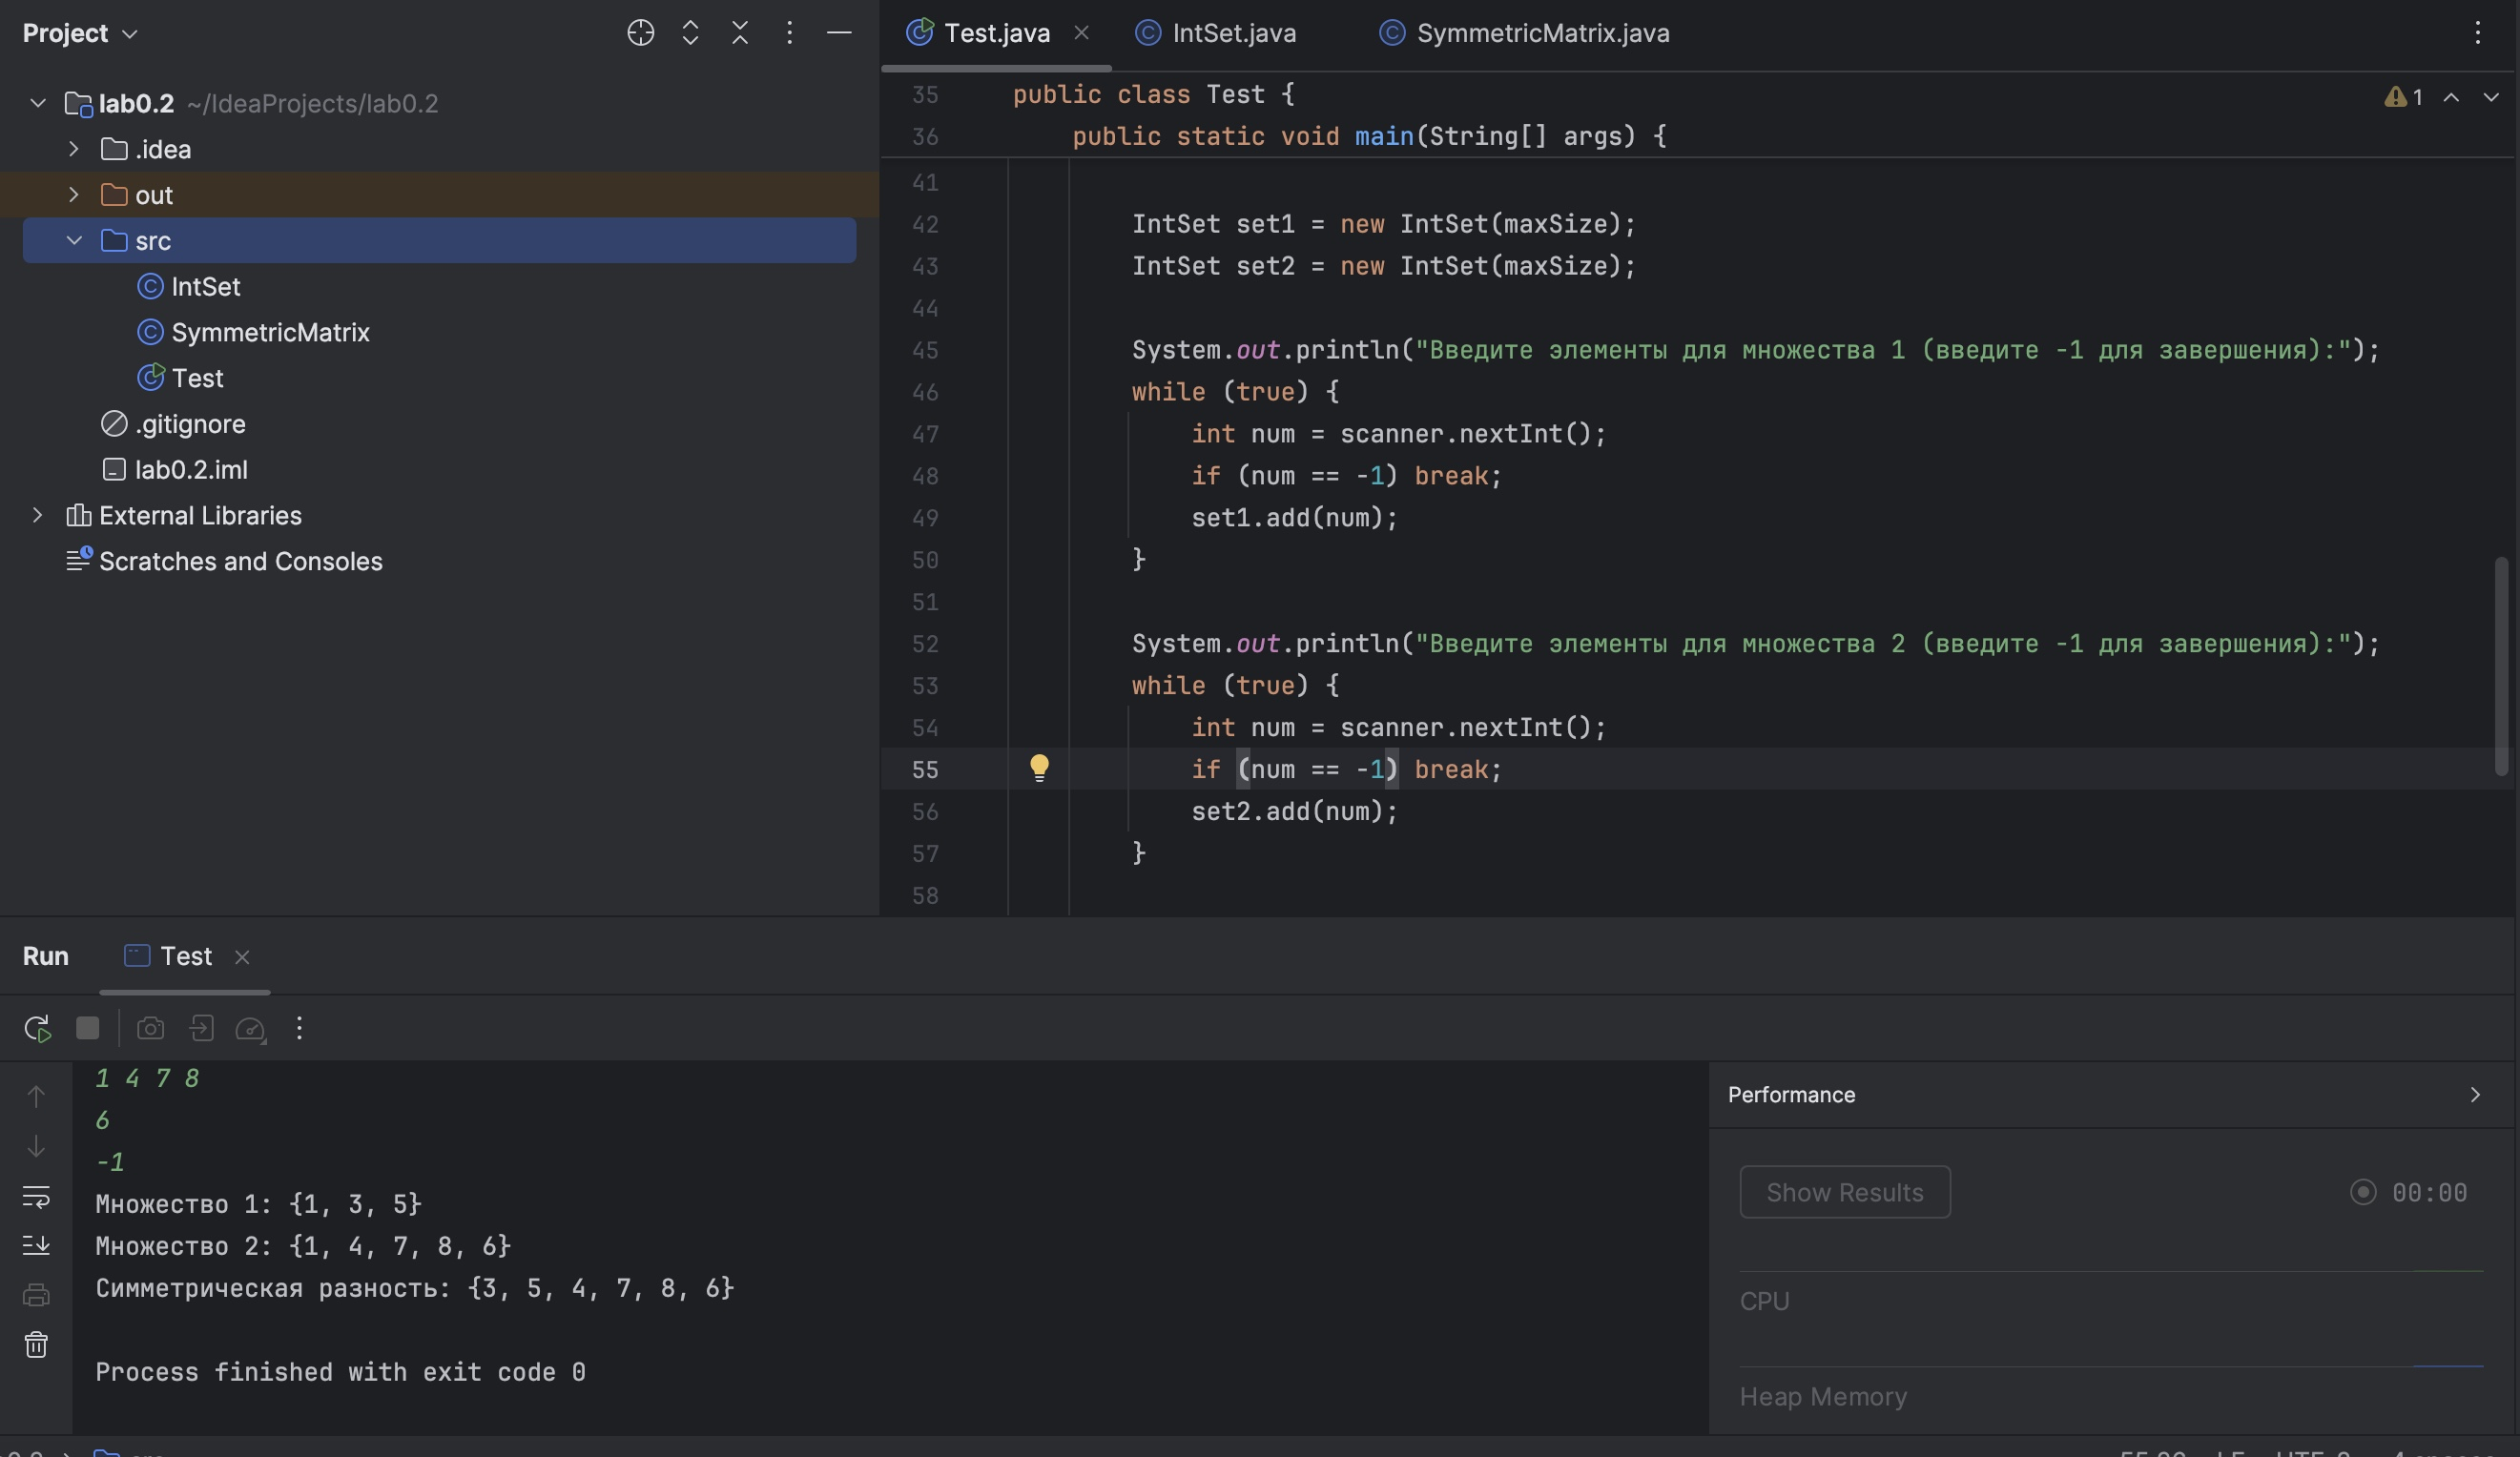
\includegraphics[width=0.8\textwidth]{фото4.jpeg}
    \captionof{figure}{Запуск программы}
\end{center}
\newpage
\section{Вывод}
В ходе выполнения лабораторной работы были разработаны два класса на языке Java: класс для работы с конечными множествами целых чисел и класс симметричных квадратных матриц. Оба класса реализуют требуемые операции, включая симметрическую разность для множеств и доступ к элементам матрицы. Для их тестирования был разработан вспомогательный класс Test, в котором реализован консольный интерфейс, позволяющий вводить данные, выполнять операции и выводить результаты. Проведённое тестирование подтвердило корректность работы реализованных методов. Таким образом, поставленные задачи успешно выполнены без использования контейнерных классов стандартной библиотеки.

\end{document}